\subsection{SVM Reduction Results}
The best model for each dataset was trained and tested on the reduced dataset obtained after applying the methods described in Section \ref{reduced-methods-sec}. Subsequently, an additional statistical analysis was carried out to determine which reduction method provided better performance.

\subsubsection{Hepatitis}
The SVM model with hyperparameters `kernel=sigmoid` and `C=100.0` was trained and tested on the reduced data samples obtained for each reduction method (DROP3, EENTH, and GCNN). The mean values of the evaluated statistical metrics are presented in Table \ref{tab:reduction_help}. Again, the Friedman test was conducted, yielding a $p$-value of 0.0057 for accuracy and 0.0210 for the F1-score. Due to these low values, the null hypothesis was rejected, and a post-hoc test was implemented. The Nemenyi test was chosen to identify specific differences between methods. Significant differences were found between EENTH and GCNN, and also between GCNN and NONE (understanding NONE as the original dataset without any reduction method), as it can be seen in the Figure \ref{fig:hep_svm_red} 

\begin{table}[h!]
\centering
\begin{tabular}{|l|c|c|c|}
\hline
\textbf{Reduction Method} & \textbf{Accuracy} & \textbf{F1 Score} & \textbf{Time (s)} \\
\hline
DROP3 & 0.79 $\pm$ 0.11 & 0.86 $\pm$ 0.07 & 0.0009 $\pm$ 0.0006 \\
\hline
EENTH & 0.85 $\pm$ 0.09 & 0.91 $\pm$ 0.06 & 0.0011 $\pm$ 0.0007 \\
\hline
GCNN  & 0.64 $\pm$ 0.13 & 0.73 $\pm$ 0.12 & 0.0014 $\pm$ 0.0007 \\
\hline
NONE  & 0.85 $\pm$ 0.10 & 0.91 $\pm$ 0.06 & 0.0011 $\pm$ 0.0004 \\
\hline
\end{tabular}
\caption{Performance metrics for different reduction methods for the SVM algorithm with kernel=sigmoid and C=100.}
\label{tab:reduction_hep}
\end{table}

\begin{figure}[t]
    \centering
    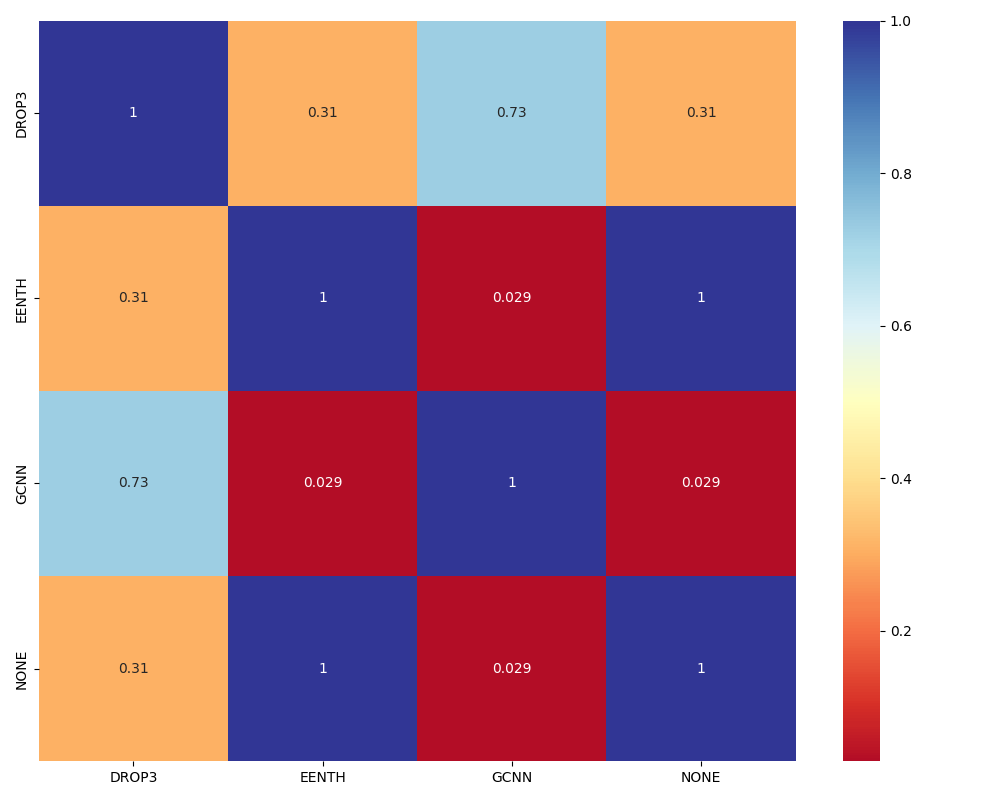
\includegraphics[width=\textwidth]{figures/svm/hepatitis/svm_results_heatmap.png}
    \caption{Normalized measure of the difference between the mean ranks of the methods.}
    \label{fig:hep_svm_red}
\end{figure}


